\documentclass{article}


\usepackage{circuitikz} %Für die Schaltpläne
\usepackage[T1]{fontenc}
\usepackage[utf8]{inputenc}
\usepackage{amsmath}
\usepackage{amssymb}
\usepackage{fancyhdr}
\usepackage{graphicx}
\usepackage{hyperref}
\usepackage{subcaption}
\usepackage{tikz}
\usepackage{cite}
\usepackage[nottoc, numbib]{tocbibind}
\usepackage{../assets/scripts/tex/color-env}
\usepackage[ngerman]{babel}


\usetikzlibrary{shapes}
    \usetikzlibrary{arrows}
    \usetikzlibrary{arrows.meta,topaths}
    \usetikzlibrary{bending}
    \usetikzlibrary{calc}
\title{Elektrotechnik 1 Praktikum 1}


\usepackage[
  includehead,
  headheight = 17mm,
  footskip = \dimexpr\headsep+\ht\strutbox\relax,
  tmargin = 0mm,
  bmargin = \dimexpr17mm+2\ht\strutbox\relax,
]{geometry}

\usepackage{anyfontsize}

\usepackage{xcolor}

\definecolor{DarkGreenBlue}{HTML}{264653}
\definecolor{LightGreenBlue}{HTML}{2A9D8F}
\definecolor{LightOrange}{HTML}{E9C46A}
\definecolor{DarkOrange}{HTML}{F4A261}
\definecolor{RedOrange}{HTML}{E76F51}
\definecolor{BrightRed}{HTML}{D62828}
\definecolor{DeepBlue}{HTML}{003049}



\pagestyle{fancy}
\fancyhead[L]{\leftmark}
\fancyhead[R]{}
\fancyfoot[L]{}
\fancyfoot[C]{\thepage}
\fancyfoot[R]{
\includegraphics[scale=0.2]{../assets/images/haw.jpg}}
\renewcommand\headrulewidth{0.5pt}


\begin{document}


\thispagestyle{empty}
\begin{tikzpicture}[remember picture,overlay]

  \fill[DeepBlue] (current page.south west) rectangle (current page.north east);

  \begin{scope}

    \foreach \i in {2.5,...,22}
      {
        \node[rounded corners, DeepBlue!90,draw ,regular polygon, regular polygon sides=6, minimum size=\i cm, ultra thick] at ($(current page.west)+(2.5,-5)$) {} ;
      }

  \end{scope}

  \node[rounded corners,fill=DeepBlue!95,text =DeepBlue!5,regular polygon,regular polygon sides=6, minimum size=2.5 cm,inner sep=0,ultra thick] at ($(current page.west)+(2.5,-5)$) {\LARGE \bfseries 2020};

  \foreach \i in {0.5,...,22}
    {
      \node[rounded corners,DeepBlue!90,draw,regular polygon,regular polygon sides=6, minimum size=\i cm,ultra thick] at ($(current page.north west)+(2.5,0)$) {} ;
    }

  \foreach \i in {0.5,...,22}
    {
      \node[rounded corners,DeepBlue!98,draw,regular polygon,regular polygon sides=6, minimum size=\i cm,ultra thick] at ($(current page.north east)+(0,-9.5)$) {} ;
    }

  \foreach \i in {12}
    {
      \node[fill = DeepBlue,rounded corners,draw=DeepBlue,regular polygon,regular polygon sides=6, minimum size=\i cm,ultra thick] at ($(current page.south east)+(-0.2,-0.45)$) {} ;
    }


  \foreach \i in {21,...,6}
    {
      \node[DeepBlue!95,rounded corners,draw,regular polygon,regular polygon sides=6, minimum size=\i cm,ultra thick] at ($(current page.south east)+(-0.2,-0.45)$) {} ;
    }

  \node[left,DeepBlue!5,minimum width=0.625*\paperwidth,minimum height=3cm, rounded corners] at ($(current page.north east)+(0,-9.5)$){{\fontsize{25}{30} \selectfont \bfseries DI - Praktikum 1}};

  \node[left,DeepBlue!10,minimum width=0.625*\paperwidth,minimum height=2cm, rounded corners] at ($(current page.north east)+(0,-11)$){{\huge \textit{Fehlersichere Übertragung und Speicherung}}};

  \node[left,DeepBlue!5,minimum width=0.625*\paperwidth,minimum height=2cm, rounded corners] at ($(current page.north east)+(0,-13)$){{\Large \textsc{Florian Tietjen\hspace{0.5cm}Eric Antosch}}};

\end{tikzpicture}

\newpage


\tableofcontents

\listoffigures

\newpage

\section{Fehlersichere Übertragung und Speicherung von Daten}

\begin{task}
  TIn diesem Praktikumsversuch geht es darum, die Übertragung und Speicherung einfacher Daten innerhalb von System zu untersuchen und zu verstehen. Dabei wollen wir nicht nur eine theoretische Betrachtung eines Paritätsgenerators betrachten, sondern diesen auch innerhalb von Xilinx Vivado beschreiben und simulieren.
\end{task}

\subsection{Vorbereitung: Schaltungaufbau}

\subsubsection{Sender}

\begin{figure}[h]
  \centering
  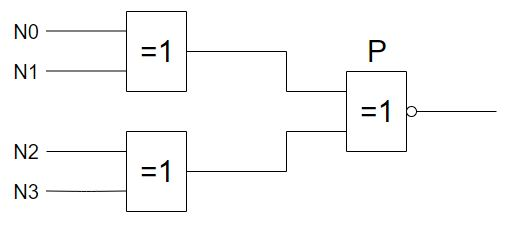
\includegraphics[width=\textwidth]{../assets/images/DI1/SenderSchalt.png}
  \caption{Schaltbild des Senders}
  \label{fig:schalt1}
\end{figure}

Wir erstellen zunächst ein Schaltbild eines Senders, welche nur ungerade Paritätsbits zulässt. Dabei gilt zu beachten, dass, im Gegensatz zu einem Sender, der gerade Paritätsbits zulässt, das letzte XOR-Gatter negiert ist und nun zu einem XNOR-Gatter wird.
\begin{figure}[h]
  \centering
  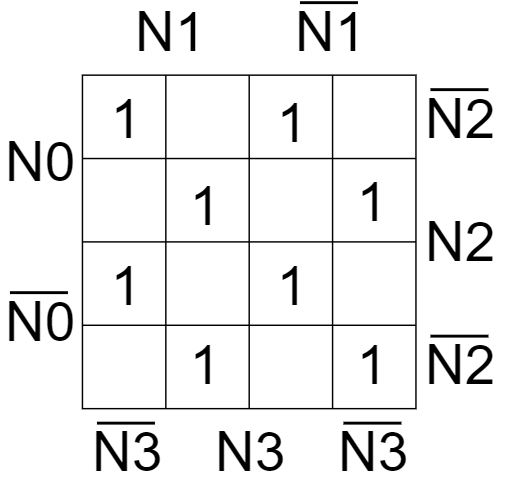
\includegraphics[width=0.3\textwidth]{../assets/images/DI1/SenderKV.png}
  \caption{KV-Diagramm des Senders}
  \label{fig:kv1}
\end{figure}

\newpage
\begin{table}[h]
\begin{center}
\begin{tabular}{c|c|c|c|c}
$N0$ & $N1$ & $N2$ & $N3$ & $P$ \\
\hline
0 & 0 & 0 & 0 & 1\\
0 & 0 & 0 & 1 & 0\\
0 & 0 & 1 & 0 & 0\\
0 & 0 & 1 & 1 & 1\\
0 & 1 & 0 & 0 & 0\\
0 & 1 & 0 & 1 & 1\\
0 & 1 & 1 & 0 & 1\\
0 & 1 & 1 & 1 & 0\\
1 & 0 & 0 & 0 & 0\\
1 & 0 & 0 & 1 & 1\\
1 & 0 & 1 & 0 & 1\\
1 & 0 & 1 & 1 & 0\\
1 & 1 & 0 & 0 & 1\\
1 & 1 & 0 & 1 & 0\\
1 & 1 & 1 & 0 & 0\\
1 & 1 & 1 & 1 & 1\\
\end{tabular}
\caption{Wahrheitstabelle vom ungeraden Paritätsbit}
\end{center}
\end{table}


Unter der Betrachtung der Wahrheitstabelle und des KV-Diagramms entsteht folgende bool'sche Formel:
\begin{align*}
  P = (\overline{N0} \wedge \overline{N1} \wedge \overline{N2} \wedge \overline{N3}) \vee (\overline{N0} \wedge \overline{N1} \wedge N2 \wedge N3) \vee (\overline{N0} \wedge N1 \wedge \overline{N2} \wedge N3) \vee (\overline{N0} \wedge N1 \wedge N2 \wedge \overline{N3}) \\
  \vee (N0 \wedge \overline{N1} \wedge \overline{N2} \wedge N3) \vee (N0 \wedge \overline{N1} \wedge N2 \wedge \overline{N3}) \vee (N0 \wedge N1 \wedge \overline{N2} \wedge \overline{N3}) \vee (N0 \wedge N1 \wedge N2 \wedge N3)
\end{align*}

Wir wollen diese nun einmal leicht vereinfachen, sodass wir diese auch leichter in unser Programm einbauen können:

\begin{equation}
  \label{eq:1}
  P = \overline{(N0 \oplus N1) \oplus (N2 \oplus N3)},
\end{equation}


\noindent
wobei es zu erwähnen gilt, dass $\oplus$ hier für die XOR-Verknüpfung gilt. (Diese wird auf dem Schaltplan mit $=1$ dargestellt).

\newpage
\subsubsection{Empfänger}
\begin{figure}[h]
  \centering
  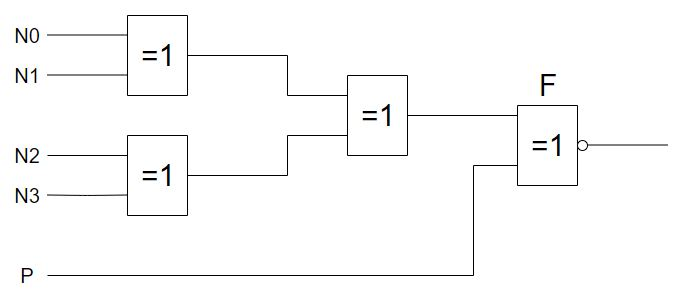
\includegraphics[width=\textwidth]{../assets/images/DI1/ReceiverSchalt.png}
  \caption{Schaltbild des Empfängersystems}
  \label{fig:schalt2}
\end{figure}

Im Empfängersystem wird nun überprüft, ob es eine gerade oder ungerade Anzahl von Einsen gibt. Im Falle, dass sich eine ungerade Anzahl an Einsen ergibt, entsteht kein Fehlersignal F (bzw. $F = 0$). Sollte es jedoch zu einem Fehler kommen, der durch verschiedene Einflüsse auf die Geräte kommen kann, und es sind nun eine gerade Anzahl an Einsen vorhanden, so entsteht ein Fehlersignal am Ausgang ($F = 1$).

\begin{figure}[h]
  \centering
  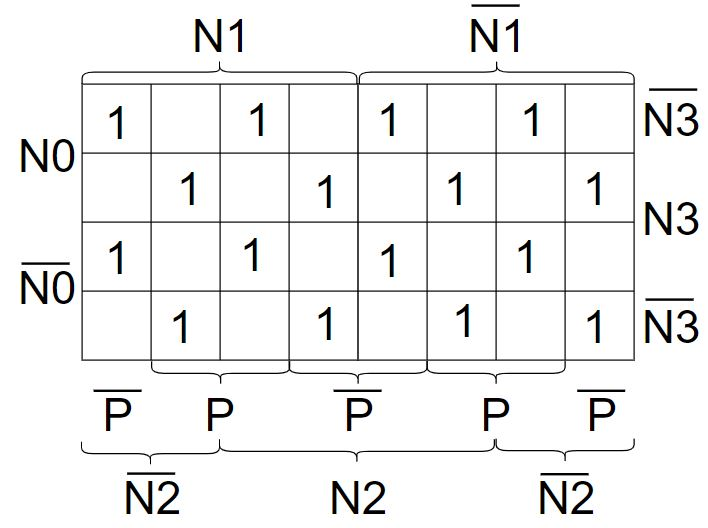
\includegraphics[width=0.4\textwidth]{../assets/images/DI1/ReceiverKV.png}
  \caption{KV-Diagramm des Empfängers}
  \label{fig:kv2}
\end{figure}

\begin{table}[h]
\begin{center}
\begin{tabular}{c|c|c|c|c|c}
$N0$ & $N1$ & $N2$ & $N3$ & $P$ & $F$ \\
\hline
0 & 0 & 0 & 0 & 1 & 0\\
0 & 1 & 1 & 0 & 1 & 0\\
0 & 1 & 0 & 0 & 1 & 1\\
1 & 0 & 1 & 0 & 0 & 1\\
\end{tabular}
\caption{Wahrheitstabelle vom ungeraden Paritätsbit}
\end{center}
\end{table}

Analog zum Sendersystem wollen wir hier auch einmal betrachten, wie sich aus dem KV-Diagramm die bool'sche Formel für den Wahrheitswert von F ergibt. (Eine vollständige Wahrheitstabelle ist im Anhang zu finden (Seite: \pageref{sec:anhang})).

\begin{align*}
 F = (\overline{N0} \wedge \overline{N1} \wedge \overline{N2} \wedge \overline{N3} \wedge \overline P) \vee (\overline{N0} \wedge \overline{N1} \wedge \overline{N2} \wedge N3\wedge P) \vee (\overline{N0} \wedge \overline{N1} \wedge N2 \wedge \overline{N3}\wedge P)\\ \vee (\overline{N0} \wedge \overline{N1} \wedge N2 \wedge N3\wedge \overline P)
 \vee (\overline{N0} \wedge N1 \wedge \overline{N2} \wedge \overline{N3} \wedge P) \vee (\overline{N0} \wedge N1 \wedge \overline{N2} \wedge N3 \wedge \overline P)\\ \vee (\overline{N0} \wedge N1 \wedge N2 \wedge \overline{N3}\wedge \overline P) \vee (\overline{N0} \wedge N1 \wedge N2 \wedge N3\wedge P)
 \vee (N0 \wedge \overline{N1} \wedge \overline{N2} \wedge \overline{N3} \wedge P)\\ \vee (N0 \wedge \overline{N1} \wedge \overline{N2} \wedge N3 \wedge \overline P) \vee (N0 \wedge \overline{N1} \wedge N2 \wedge \overline{N3} \wedge \overline P) \vee (N0 \wedge \overline{N1} \wedge N2 \wedge N3\wedge P)\\
 \vee (N0 \wedge N1 \wedge \overline{N2} \wedge \overline{N3} \wedge \overline P) \vee (N0 \wedge N1 \wedge \overline{N2} \wedge N3 \wedge P) \vee (N0 \wedge N1 \wedge N2 \wedge \overline{N3} \wedge P)\\ \vee(N0 \wedge N1 \wedge N2 \wedge N3\wedge \overline P)
\end{align*}

Auch aus dieser Formel ist es sinnvoll, eine einfachere Form zu bilden, um diese übersichtlich zu halten:

\begin{equation}
  \label{eq:2}
  F = \overline{P \oplus ((N0 \oplus N1) \oplus (N2 \oplus N3))}
\end{equation}

Mit dieser Vorbereitung steht nun der eigentlichen Beschreibung der Hardware mithilfe von VHDL und Xilinx Vivado nichts mehr im Weg.
\newpage

\subsection{Hardwarebeschreibung und -simulation mit Vivado}

\subsubsection{Source: Paritätsgenerator und Empfängersystem}

Zunächst werden die beiden Sources, der Paritätsgenerator bzw. unser Sender, und das Empfängersystem mithilfe der Hardwarebeschreibungssprache VHDL in das Projekt selbst eingepflegt:

\begin{figure}[h]
  \centering
  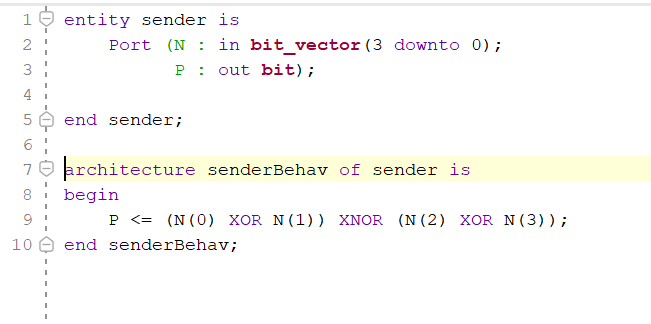
\includegraphics[width=\textwidth]{../assets/images/DI1/sendervhd.PNG}
  \caption{Sender-VHDL-Beschreibung (Paritätsgenerator)}
  \label{fig:vhd1}
\end{figure}

\begin{figure}[h]
  \centering
  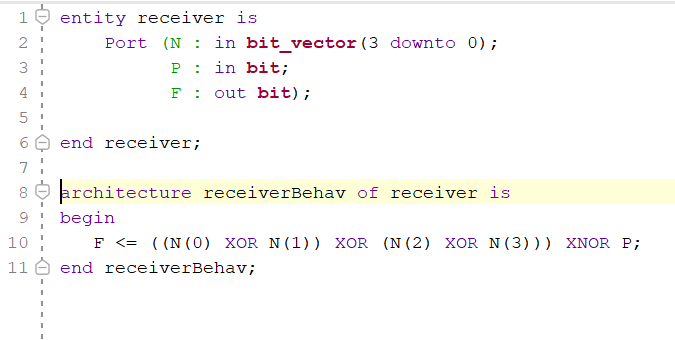
\includegraphics[width=\textwidth]{../assets/images/DI1/receivervhd.PNG}
  \caption{Empfänger-VHDL-Beschreibung}
  \label{fig:vhd2}
\end{figure}
\newpage

\subsubsection{Testbench: Paritätsgenerator und Empfängersystem}

Nachdem nun beide Bauteile erfolgreich mit VHDL beschrieben worden sind, wollen wir uns nun daran machen, die beiden Systeme mit einer entsprechenden Testbench zu simulieren. Dazu erstellen wir für jedes der Bauteile eine einzelne Datei, in der wir die Test, die später in der Simulation ablaufen sollen, beschreiben:

\begin{figure}[h]
  \centering
  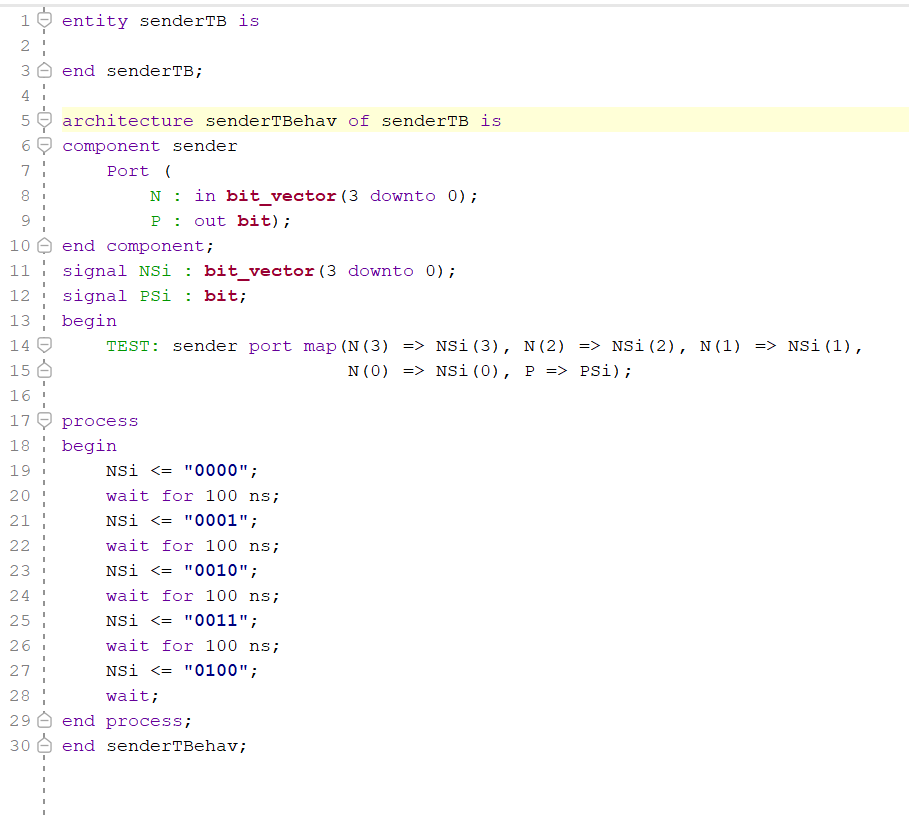
\includegraphics[width=\textwidth]{../assets/images/DI1/senderTB.PNG}
  \caption{Sender-Testbench (Paritätsgenerator)}
  \label{fig:vhdTB1}
\end{figure}

\begin{figure}[h]
  \centering
  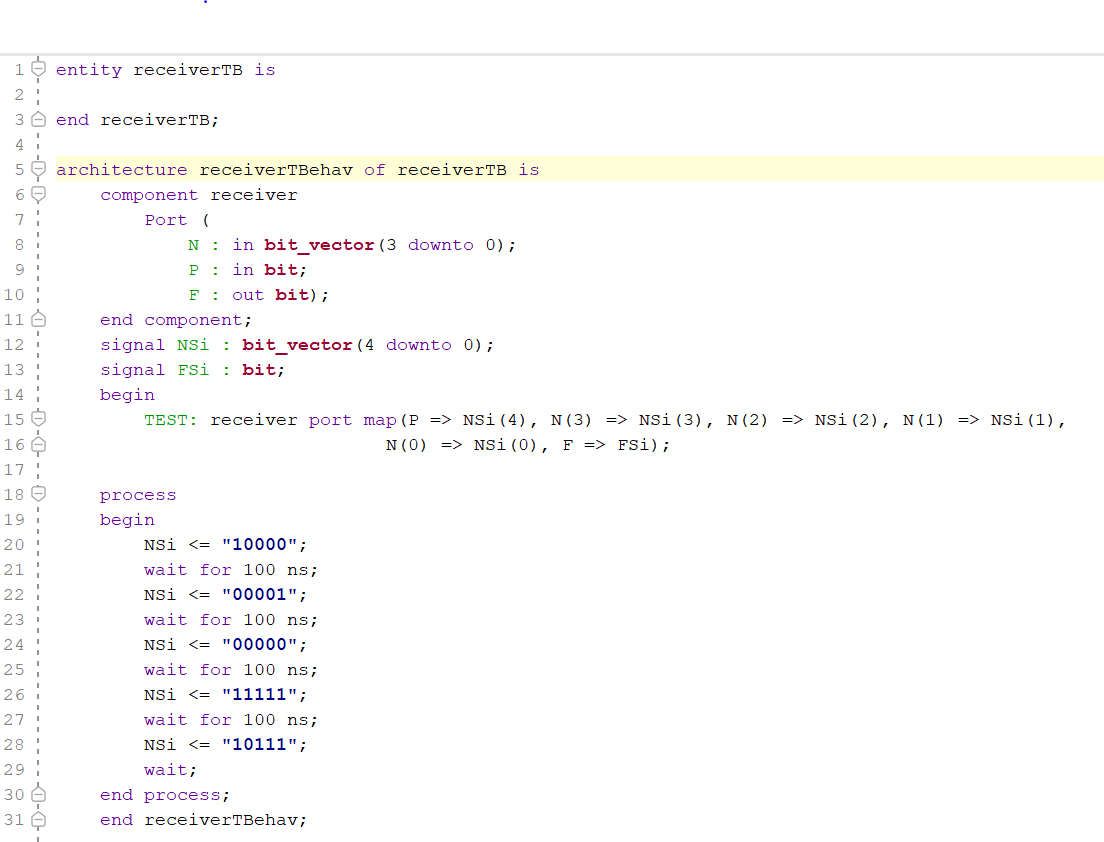
\includegraphics[width=\textwidth]{../assets/images/DI1/receiverTB.PNG}
  \caption{Empfänger-Testbench}
  \label{fig:vhdTB2}
\end{figure}
\newpage


\subsubsection{Testbench: Auswertung der Ergebnisse im Waveform-Viewer}

Im letzten Abschnitt wollen wir nun die Auswertung der Ergebnisse der Simulation aus dem Waveform-Viewer von Vivado vornehmen. Dazu betrachten wir zunächst unseren Paritätsgenerator um festzustellen, ob wir diesen richtig implementiert haben.

\begin{figure}[h]
  \centering
  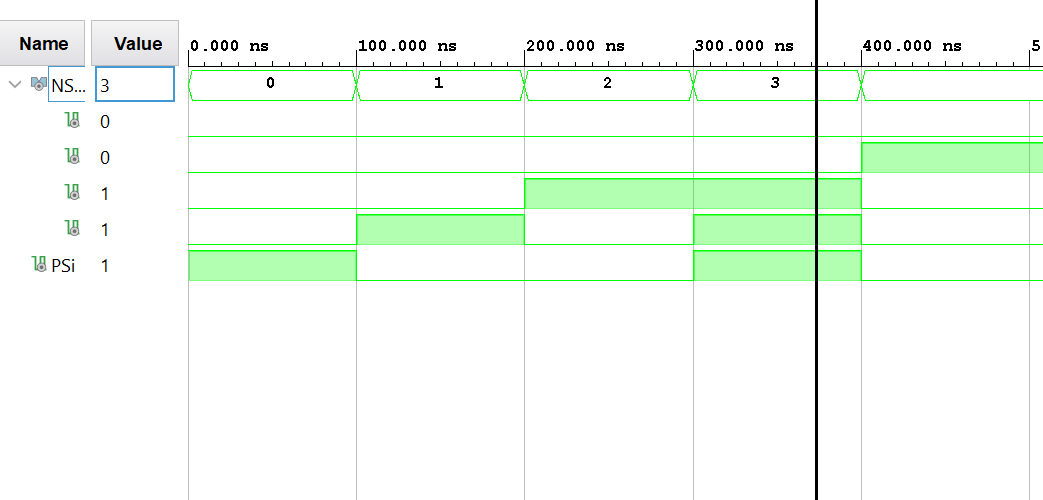
\includegraphics[width=\textwidth]{../assets/images/DI1/senderTBSim.PNG}
  \caption{Waveform des Senders (Paritätsgenerator)}
  \label{fig:wf1}
\end{figure}

Wir können gut erkennen, dass unser Paritätsgenerator das erwartete Verhalten zeigt. So wird zum Beispiel im Bereich von 0ns bis 100ns eine 1 auf das Paritätsbit (in unserem Fall PSi genannnt) gesetzt, da beide vor geschalteten XOR-Gatter eine 0 ausgeben.

\newpage
Nun wollen wir uns auch unseren Empfänger anschauen:

\begin{figure}[h]
  \centering
  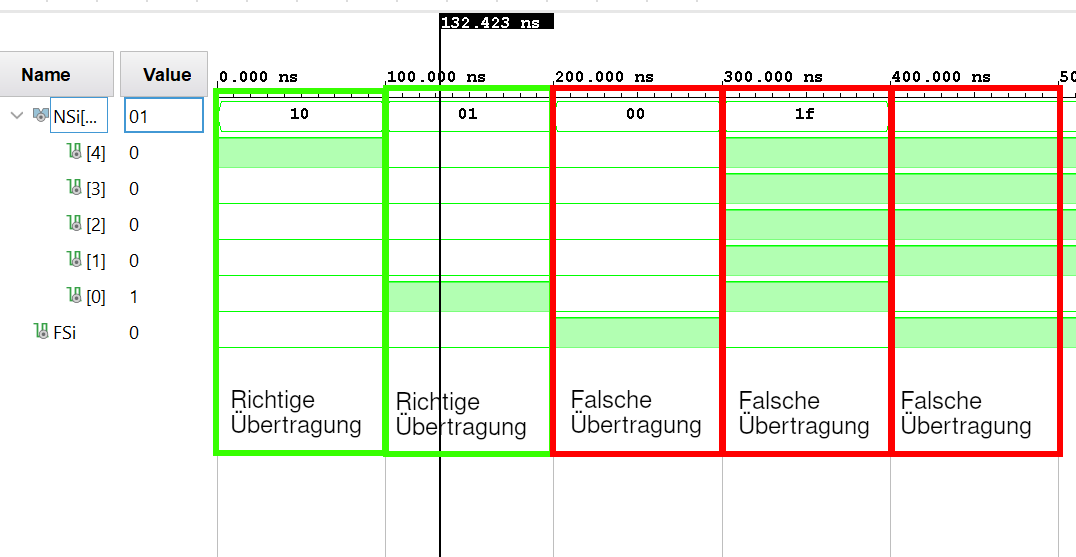
\includegraphics[width=\textwidth]{../assets/images/DI1/receiverTBSim.PNG}
  \caption{Waveform des Empfängers}
  \label{fig:wf2}
\end{figure}

Es wird deutlich, dass sich unser Sender-Empfängersystem unseren Vorstellungen entsprechend verhält. Zunächst werden zwei Übertragungen (0ns-100ns, 100ns-200ns) gemacht, die richtige Einstellungen haben. Im Bereich von 200ns-300ns liegt ein einfacher Fehler vor, der von dem Fehlersignal FSi richtig erkannt wird. Zwischen 300ns und 400ns sind jedoch zwei Fehler eingebaut, was von unserer Überprüfungsstrecke nicht korrekt erfasst wird. Im letzten Bereich ist unser Paritätssignal nicht korrekt, es entsteht erneut ein Fehler am Ausgang FSi.

\subsection{Fehler}

Es wird deutlich, dass eine einfach Paritätsüberprüfungsstrecke nicht in der Lage ist, Fehler mit gerader Anzahl zu ermitteln. Bei Fehlern mit ungerader Anzahl jedoch, schlägt das Signal aus und der Fehler könnte von aus behoben werden.

\subsection{Freiheiten der Verbesserung der Übertragungsstrecke}

Es liegt nahe, einer wichtigen Übertragungsstrecke von Daten mehrere Sicherheitssysteme zu verleihen. So würde es sich beispielsweise anbieten, verschiedene Paritätssignale in eine Übertragungsstrecke einzubauen, um auch Fehler abzufangen, die dann in gerade Anzahl auftauchen. Dies verkompliziert den Aufbau einer solchen Schaltung auch nur im bedingten Maße.

\section{Fazit}

Es ist eindeutig zu erkennen, dass eine Paritätsprüfung zur Sicherstellung der Datensicherheit nur einen eingeschränkten Schutz gegen Fehler bietet. Es gilt sich daher zu überlegen, dieses System mithilfe von Erweiterungen gegen größere Bandbreite an Fehlern abzusichern.
Während der Durchführung des Praktikums ist vor allen Dingen die steile Lernkurve sowohl von VHDL als auch Vivado aufgefallen. Es ist zu Beginn sehr viel Zeit in die Einarbeitung in die Programmierweise und das Programm selbst geflossen, sowie in das Beheben von Fehlern, die sich als Flüchtigkeits- oder Unwissenheitsfehler entpuppt haben. Vor Beginn des nächsten Praktikums bietet es sich daher an, mehr über VHDL als Sprache und das Programm Xilinx Vivado zu lernen.

\newpage
\section[Anhang]{Anhang}
\label{sec:anhang}
\begin{table}[h]
  \begin{center}
\begin{tabular}{c|c|c|c|c|c}
  $N0$ & $N1$ & $N2$ & $N3$ & $P$ & $F$ \\
  \hline
  0 & 0 & 0 & 0 & 0 & 1\\
  0 & 0 & 0 & 0 & 1 & 0\\
  0 & 0 & 0 & 1 & 0 & 0\\
  0 & 0 & 0 & 1 & 1 & 1\\
  0 & 0 & 1 & 0 & 0 & 0\\
  0 & 0 & 1 & 0 & 1 & 1\\
  0 & 0 & 1 & 1 & 0 & 1\\
  0 & 0 & 1 & 1 & 1 & 0\\
  0 & 1 & 0 & 0 & 0 & 0\\
  0 & 1 & 0 & 0 & 1 & 1\\
  0 & 1 & 0 & 1 & 0 & 0\\
  0 & 1 & 0 & 1 & 1 & 1\\
  0 & 1 & 1 & 0 & 0 & 1\\
  0 & 1 & 1 & 0 & 1 & 0\\
  0 & 1 & 1 & 1 & 0 & 0\\
  0 & 1 & 1 & 1 & 1 & 1\\
  1 & 0 & 0 & 0 & 0 & 0\\
  1 & 0 & 0 & 0 & 1 & 1\\
  1 & 0 & 0 & 1 & 0 & 1\\
  1 & 0 & 0 & 1 & 1 & 0\\
  1 & 0 & 1 & 0 & 0 & 1\\
  1 & 0 & 1 & 0 & 1 & 0\\
  1 & 0 & 1 & 1 & 0 & 0\\
  1 & 0 & 1 & 1 & 1 & 1\\
  1 & 1 & 0 & 0 & 0 & 1\\
  1 & 1 & 0 & 0 & 1 & 0\\
  1 & 1 & 0 & 1 & 0 & 0\\
  1 & 1 & 0 & 1 & 1 & 1\\
  1 & 1 & 1 & 0 & 0 & 0\\
  1 & 1 & 1 & 0 & 1 & 1\\
  1 & 1 & 1 & 1 & 0 & 1\\
  1 & 1 & 1 & 1 & 1 & 0\\
\end{tabular}
\caption{Wahrheitstabelle vom Empfänger}
\end{center}
\end{table}


\end{document}
